\chapter{Laboratorium 6}
\label{cha:Lab006}
\makeatletter


% *********************************************************************
% w poniższej metryczce należy uzupełnić informacje o:
% - temacie ćwiczenia
% - numer ćwiczenia
% - numer grupy laboratoryjnej
% - numer zespołu
% - datę wykonania ćwiczenia oraz oddania ćwiczenia.
% *********************************************************************

\begin{table}[H]
    \centering
    \renewcommand{\tabularxcolumn}[1]{m{#1}}  % Dostosowanie kolumny do zawartości
    \newcolumntype{C}{>{\centering\arraybackslash}X}
    \begin{tabularx}{\linewidth}{|C|C|}
        \hline
        \multicolumn{2}{|c|}{\makecell{\textbf{\Large{Biometryczne Systemy Zabezpieczeń}} \\ \textbf{Ćwiczenia Laboratoryjne}}} \\ \hline
        \multicolumn{1}{|l|}{Temat}                    &              OBRAZY DAKTYLOSKOPIJNE TOKENIZACJA- METODA PROSTA I GRAFOWA , TOKENIZACJA TĘCZÓWKI OKA ALGORYTM JOHNA DAUGMANA            \\ \hline
        \multicolumn{1}{|l|}{Ćwiczenie nr:}                    &      06                   \\ \hline
        \multicolumn{1}{|l|}{Autorzy:}                         &   \@author                              \\ \hline
        \multicolumn{1}{|l|}{Grupa laboratoryjna}                       &       02               \\ \hline
        \multicolumn{1}{|l|}{Zespół nr. }                       &    XX                  \\ \hline
        \multicolumn{1}{|l|}{Data wykonana ćwiczenia}         &  06.05.2025     \\ \hline
        \multicolumn{1}{|l|}{Data oddania ćwiczenia  }         &   13.05.2025     \\ \hline
    \end{tabularx}
\end{table}


\section{Cel ćwiczenia}

Celem laboratorium jest zrozumienie procesu tokenizacji w kontekście danych biometrycznych oraz
praktyczna implementacja algorytmów do ekstrakcji cech z obrazów daktyloskopijnych (minucje) oraz
porównanie prostych i grafowych metod dopasowania tokenów. Zastosowanie algorytmu Johna
Daugmana do tokenizacji pola tęczówki oka oraz wyznaczanie miary podobieństwa poprzez obliczenie
dystansu Hamminga.

\section{Wstęp teoretyczny}

Obrazy daktyloskopijne (ang. \textit{fingerprint images}) to obrazy przedstawiające wzór linii papilarnych palca, składający się z charakterystycznych grzbietów (\textit{ridge}) i dolin (\textit{valley}). Te lokalnie periodyczne struktury są unikalne dla każdej osoby i stanowią podstawę systemów biometrycznych opartych na rozpoznawaniu odcisków palców.

Etapy przetwarzania obrazu daktyloskopijnego można zestawić w następującej kolejności:

\begin{enumerate}
	\item \textbf{Pozyskiwanie obrazu (Image Acquisition)} – rejestracja obrazu odcisku palca przy użyciu skanera optycznego, pojemnościowego, ultradźwiękowego itp.
	\item \textbf{Wstępne przetwarzanie (Preprocessing)} – korekcja kontrastu, usuwanie szumu, poprawa jakości obrazu.
	\item \textbf{Wzmocnienie i filtrowanie (Enhancement \& Filtering)} – zastosowanie filtrów (np. Gabora) w celu uwydatnienia struktury linii papilarnych.
	\item \textbf{Binaryzacja i ścienianie (Binarization \& Thinning)} – przekształcenie obrazu do formy binarnej (0/1) i redukcja grubości linii do 1 piksela.
	\item \textbf{Ekstrakcja minucji (Minutiae Extraction)} – wykrywanie punktów charakterystycznych, takich jak zakończenia linii (\textit{ending}) czy rozwidlenia (\textit{bifurcation}).
\end{enumerate}

\subsection*{Model matematyczny obrazu daktyloskopijnego}

Obraz odcisku palca można opisać jako funkcję:
\begin{equation}
	I(x, y): \mathbb{Z}^2 \rightarrow [0,255]
\end{equation}
gdzie $I(x,y)$ oznacza wartość jasności piksela o współrzędnych $(x,y)$. Typowy obraz daktyloskopijny ma rozmiar np. $512 \times 512$ pikseli i rozdzielczość 500~dpi, co odpowiada ok. 19,7~$\mu$m/piksel.

Wzorce linii papilarnych są lokalnie okresowe — grzbiety i doliny mają charakterystyczne częstotliwości przestrzenne. Filtrowanie w dziedzinie częstotliwości pozwala na:
\begin{itemize}
	\item zwiększenie kontrastu grzbietów,
	\item tłumienie szumów,
	\item poprawę jakości detekcji minucji.
\end{itemize}

\subsection*{Filtr Gabora}

Filtr Gabora jest często używanym narzędziem do analizy tekstury w obrazach biometrycznych. Łączy w sobie lokalizację przestrzenną (funkcja Gaussa) i selektywność częstotliwościową (fala sinusoidalna).

Postać filtru Gabora:
\begin{equation}
	G(x, y) = \exp\left( -\frac{x'^2 + \gamma^2 y'^2}{2\sigma^2} \right) \cdot \cos\left(2\pi \frac{x'}{\lambda} + \phi \right)
\end{equation}
gdzie:
\begin{align}
	x' &= x \cos\theta + y \sin\theta \\
	y' &= -x \sin\theta + y \cos\theta
\end{align}

Parametry:
\begin{itemize}
	\item $\lambda$ – długość fali (częstotliwość grzbietu),
	\item $\theta$ – orientacja lokalna grzbietów,
	\item $\phi$ – przesunięcie fazowe (zwykle 0 lub $\pi/2$),
	\item $\sigma$ – skala funkcji Gaussa (rozmycie),
	\item $\gamma$ – eliptyczność filtru.
\end{itemize}

Filtracja obrazu odcisku palca:
\begin{equation}
	I'(x, y) = I(x, y) * G_{\theta(x,y), \lambda(x,y)}(x, y)
\end{equation}

Zastosowanie filtru zwiększa kontrast grzbietów, redukuje szum i poprawia ekstrakcję minucji.

\subsection*{Binaryzacja i szkieletyzacja}

Celem binarnej segmentacji (np. metodą Otsu) jest uzyskanie obrazu 0-1, gdzie linie papilarne są reprezentowane jako ciągi pikseli. Następnie stosuje się \textbf{ścienianie} (ang. \textit{thinning}) w celu sprowadzenia szerokich linii do ich szkieletu o szerokości jednego piksela. Dzięki temu możliwa jest precyzyjna detekcja cech takich jak rozwidlenia i zakończenia linii.

\subsection*{Ekstrakcja i tokenizacja minucji}

Minucje to charakterystyczne punkty na liniach papilarnych:
\begin{itemize}
	\item zakończenia linii (ending),
	\item rozwidlenia (bifurcation).
\end{itemize}

Każda minucja może być opisana trójkątem $(x, y, \theta)$:
\begin{equation}
	M = [x, y, \theta]
\end{equation}

Zestaw takich punktów stanowi token biometryczny. Może on być wykorzystany w systemach dopasowujących, np. poprzez porównanie pozycji i orientacji lub przez analizę struktury grafowej zależności między minucjami.

\subsection*{Usuwanie fałszywych minucji}

Fałszywe minucje mogą powstać w wyniku zakłóceń, obciętych krawędzi obrazu lub niedoskonałości w przetwarzaniu morfologicznym. W celu ich eliminacji stosuje się:
\begin{itemize}
	\item heurystyki geometryczne (odległość, orientacja, pozycja),
	\item ocenę jakości minucji,
	\item metody uczenia maszynowego do klasyfikacji prawdziwych/fałszywych minucji.
\end{itemize}


\section{Opis wykorzystywanego oprogramowania i narzędzi}

\section{Zadania do wykonania samodzielnego}

\subsection{Zadanie 1}

\subsubsection{Treść}

Wykonaj tokenizację wybranej pary obrazów daktyloskopijnych i wyznacz podobieństwa zestawów
wyodrębnionych minucji z wykorzystaniem metody prostej oraz grafowej. Porównaj skuteczność obu
metod.

\subsubsection{Przykładowy program}

\lstinputlisting[style= matlabStyle, caption= Algorytm rozkładu w szereg Fouriera, label=Lab006_l1]{src/Lab006/zadanie1.m}

\subsubsection{Obrazy}

\begin{figure}[H]
	\centering
	\begin{subfigure}[t]{0.45\linewidth}
		\centering
		
\includegraphics[width=\linewidth]{src/lab006/zad1results.png}
		\label{fig:lab6z1_finger1}
	\end{subfigure}
	\hfill
	\begin{subfigure}[t]{0.45\linewidth}
		\centering
		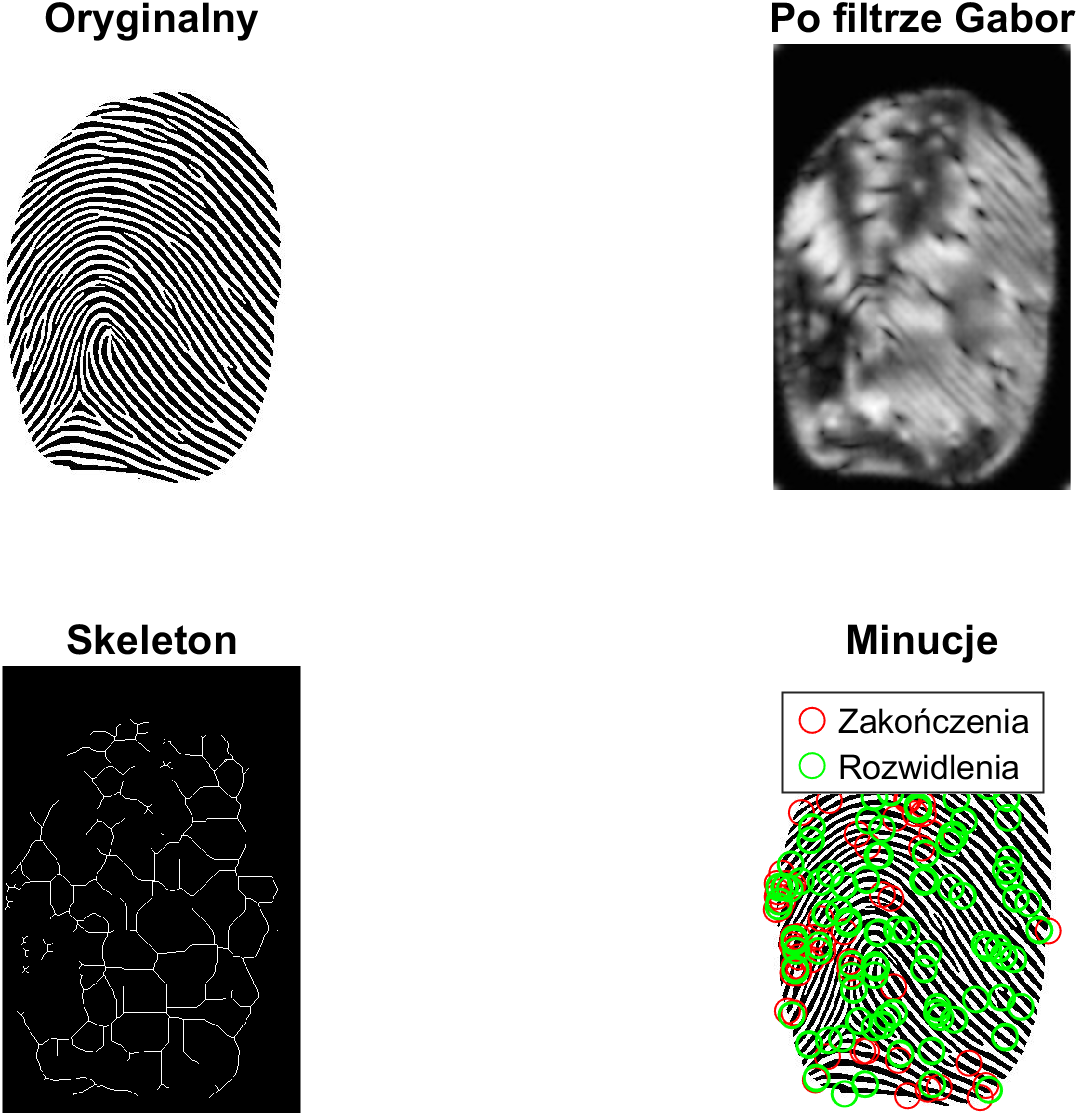
\includegraphics[width=\linewidth]{src/Lab006/zad2results.png}
		\label{fig:lab6z1_finger2}
	\end{subfigure}
\end{figure}

\subsection{Zadanie 2}

\subsubsection{Treść}

Wykonaj tokenizację wybranej podanego zestawu obrazów tęczówki oka i wyznacz dla każdej pary
dystans Hamminga HD. Oceń otrzymane wyniki ze względu na podobieństwo i poziom okluzji pola
tęczówki.

\subsubsection{Przykładowy program}

\lstinputlisting[style= matlabStyle, caption= Algorytm rozkładu w szereg Fouriera, label=Lab006_l2]{src/Lab006/zadanie2.m}

\subsubsection{Obrazy}

% --- Grupa 1: Wyryte tęczówki ---
\begin{figure}[H]
	\centering
	\begin{subfigure}[t]{0.3\linewidth}
		
\includegraphics[width=\linewidth]{src/lab006/output/iris_detected_01.png}
		\caption{Obraz 1}
		\label{fig:lab6z2_iris_detected1}
	\end{subfigure}
	\hfill
	\begin{subfigure}[t]{0.3\linewidth}
		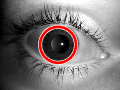
\includegraphics[width=\linewidth]{src/Lab006/output/iris_detected_02.png}
		\caption{Obraz 2}
		\label{fig:lab6z2_iris_detected2}
	\end{subfigure}
	\hfill
	\begin{subfigure}[t]{0.3\linewidth}
		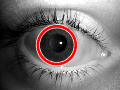
\includegraphics[width=\linewidth]{src/Lab006/output/iris_detected_03.png}
		\caption{Obraz 3}
		\label{fig:lab6z2_iris_detected3}
	\end{subfigure}
	\caption{Wyryte tęczówki}
\end{figure}

% --- Grupa 2: Znormalizowane tęczówki ---
\begin{figure}[H]
	\centering
	\begin{subfigure}[t]{0.3\linewidth}
		
\includegraphics[width=\linewidth]{src/lab006/output/iris_normalized_01.png}
		\caption{Normalizacja 1}
		\label{fig:lab6z2_iris_normalized1}
	\end{subfigure}
	\hfill
	\begin{subfigure}[t]{0.3\linewidth}
		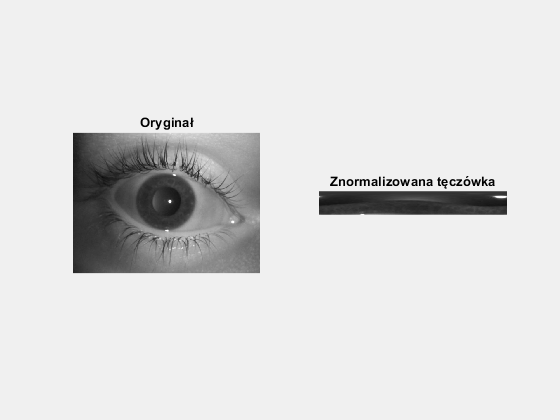
\includegraphics[width=\linewidth]{src/Lab006/output/iris_normalized_02.png}
		\caption{Normalizacja 2}
		\label{fig:lab6z2_iris_normalized2}
	\end{subfigure}
	\hfill
	\begin{subfigure}[t]{0.3\linewidth}
		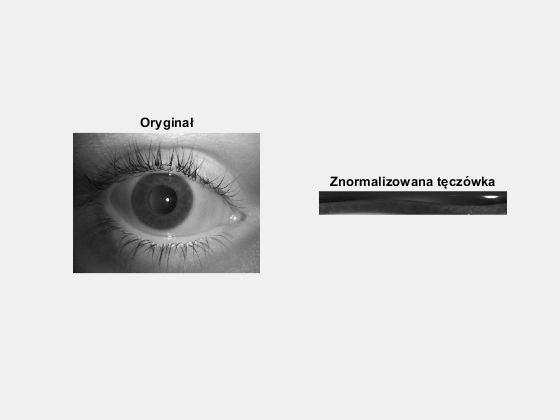
\includegraphics[width=\linewidth]{src/Lab006/output/iris_normalized_03.png}
		\caption{Normalizacja 3}
		\label{fig:lab6z2_iris_normalized3}
	\end{subfigure}
	\caption{Znormalizowane tęczówki}
\end{figure}

% --- Grupa 3: Macierz Hamminga ---
\begin{figure}[H]
	\centering
	
\includegraphics[width=0.5\linewidth]{src/lab006/output/hamming_matrix.png}
	\caption{Macierz dystansu Hamminga}
	\label{fig:lab6z2_matrix}
\end{figure}


\section{Wnioski}

Na podstawie przeprowadzonych eksperymentów można stwierdzić, że:

W normalizacji
\begin{itemize}
	\item Normalizacja obrazu do postaci prostokątnej pozwoliła na wyrównanie różnic wynikających z położenia i wielkości tęczówki w obrazach wejściowych.
	\item Uzyskane postacie normalizowane charakteryzowały się spójną strukturą, co umożliwiło dalsze przetwarzanie.
	\item Segmentacja oparta na założeniu środkowego położenia źrenicy okazała się wystarczająca przy obrazach dobrze wycentrowanych, jednak może nie sprawdzać się w bardziej realistycznych scenariuszach (np. zepsute detekcje, okluzje powiek).
\end{itemize}

W tokenizacji
\begin{itemize}
	\item Tokenizacja z użyciem filtrów Gabora pozwoliła uzyskać binarne wzorce reprezentujące strukturę tęczówki.
	\item Macierz dystansu Hamminga wykazała wyraźne różnice między parami obrazów: najniższe wartości wskazywały na wysokie podobieństwo, natomiast wartości bliskie 0.5 sugerowały brak zgodności (lub silną okluzję).
	\item Okluzje fragmentów tęczówki (np. rzęsy, powieki) znacząco wpływają na zwiększenie dystansu Hamminga, ponieważ maski nie zawsze skutecznie eliminują szumy z tokenów.
	\item Pomimo uproszczeń w modelu, metoda pozwala skutecznie odróżnić obrazy tej samej tęczówki od różnych.
\end{itemize}

Przeprowadzony proces dowodzi, że nawet uproszczona segmentacja i normalizacja umożliwiają wykonanie skutecznej ekstrakcji cech biometrycznych. Dystans Hamminga dobrze sprawdza się jako miara podobieństwa binarnych tokenów i potwierdza, że metoda jest odporna na drobne zakłócenia, choć jej skuteczność zależy od jakości segmentacji i maskowania zakłóceń.